% ---------------------------------------------------------------------------
% Author guideline and sample document for EG publication using LaTeX2e input
% D.Fellner, v1.13, April 29, 2009

\documentclass{egpubl}
\usepackage{sigrad13}

% --- for  Annual CONFERENCE
% \ConferenceSubmission % uncomment for Conference submission
% \ConferencePaper      % uncomment for (final) Conference Paper
% \STAR                 % uncomment for STAR contribution
% \Tutorial             % uncomment for Tutorial contribution
% \ShortPresentation    % uncomment for (final) Short Conference Presentation
%
% --- for  CGF Journal
% \JournalSubmission    % uncomment for submission to Computer Graphics Forum
% \JournalPaper         % uncomment for final version of Journal Paper
%
% --- for  EG Workshop Proceedings
\WsSubmission    % uncomment for submission to EG Workshop
% \WsPaper         % uncomment for final version of EG Workshop contribution
%
 \electronicVersion % can be used both for the printed and electronic version

% !! *please* don't change anything above
% !! unless you REALLY know what you are doing
% ------------------------------------------------------------------------

% for including postscript figures
% mind: package option 'draft' will replace PS figure by a filname within a frame
\ifpdf \usepackage[pdftex]{graphicx} \pdfcompresslevel=9
\else \usepackage[dvips]{graphicx} \fi

\PrintedOrElectronic

% prepare for electronic version of your document
\usepackage{t1enc,dfadobe}

\usepackage{egweblnk}
\usepackage{subfigure}
\usepackage{algorithmic}
\usepackage{algorithm}
\usepackage{cite}

% For backwards compatibility to old LaTeX type font selection.
% Uncomment if your document adheres to LaTeX2e recommendations.
% \let\rm=\rmfamily    \let\sf=\sffamily    \let\tt=\ttfamily
% \let\it=\itshape     \let\sl=\slshape     \let\sc=\scshape
% \let\bf=\bfseries

% end of prologue

\renewcommand{\algorithmicrequire}{\textbf{Input:}}
\renewcommand{\algorithmicensure}{\textbf{Output:}}
\newcommand{\red}[1]{{\color{red}{#1}}}
\newcommand{\fix}[1]{\red{\emph{#1}}}
\newcommand{\Fix}[1]{\begin{itemize} \renewcommand\labelitemi{\red{--}} \item \red{#1} \end{itemize}}

% ---------------------------------------------------------------------
% EG author guidelines plus sample file for EG publication using LaTeX2e input
% D.Fellner, v1.17, Sep 23, 2010


%\title[Spherical Raycasting]{Raycasting of Datasets with Spherical Symmetry}
\title[Spherical Raycasting]{Towards Raycasting of Datasets with Inherent Spherical Symmetry}
% Spherical Coordinates


% For anonymous conference submission, please enter your SUBMISSION ID.
%\author[102]{Submission ID 102}
\author[A. Bock et al.]{Alexander Bock$^{1}$, Martin T\"ornros$^2$, Anders Ynnerman$^{1}$, and Timo Ropinski$^{1}$ \\
${^1}$ Scientific Visualization Group, Link\"oping University\\
${^2}$ Goddard Space Flight Center, NASA
}
 
% ------------------------------------------------------------------------

% if the Editors-in-Chief have given you the data, you may uncomment
% the following five lines and insert it here
%
% \volume{27}   % the volume in which the issue will be published;
% \issue{1}     % the issue number of the publication
% \pStartPage{1}      % set starting page


%-------------------------------------------------------------------------
\begin{document}

\teaser{
	\centering
	\subfigure[Spherical]{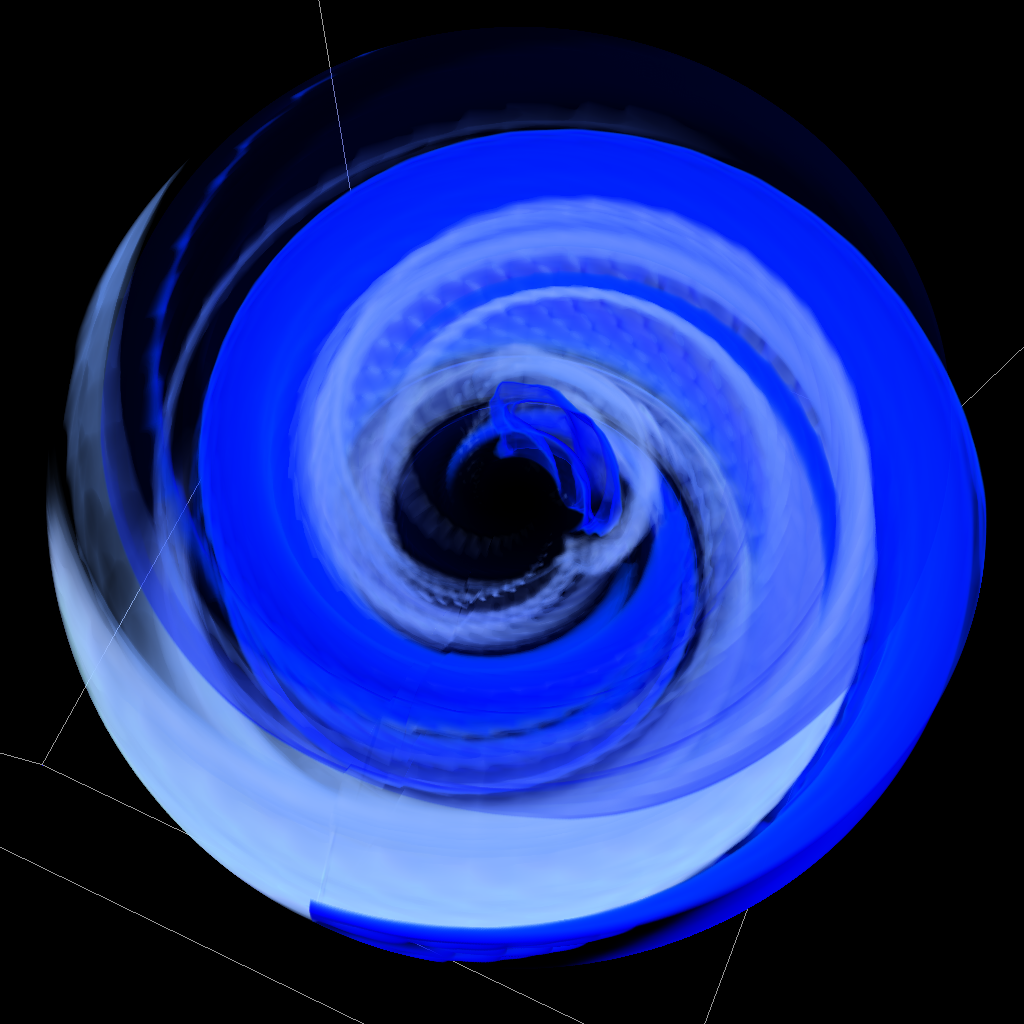
\includegraphics[width=0.32\linewidth]{figures/sphere_64.png}}
	\subfigure[Resampled (same size)]{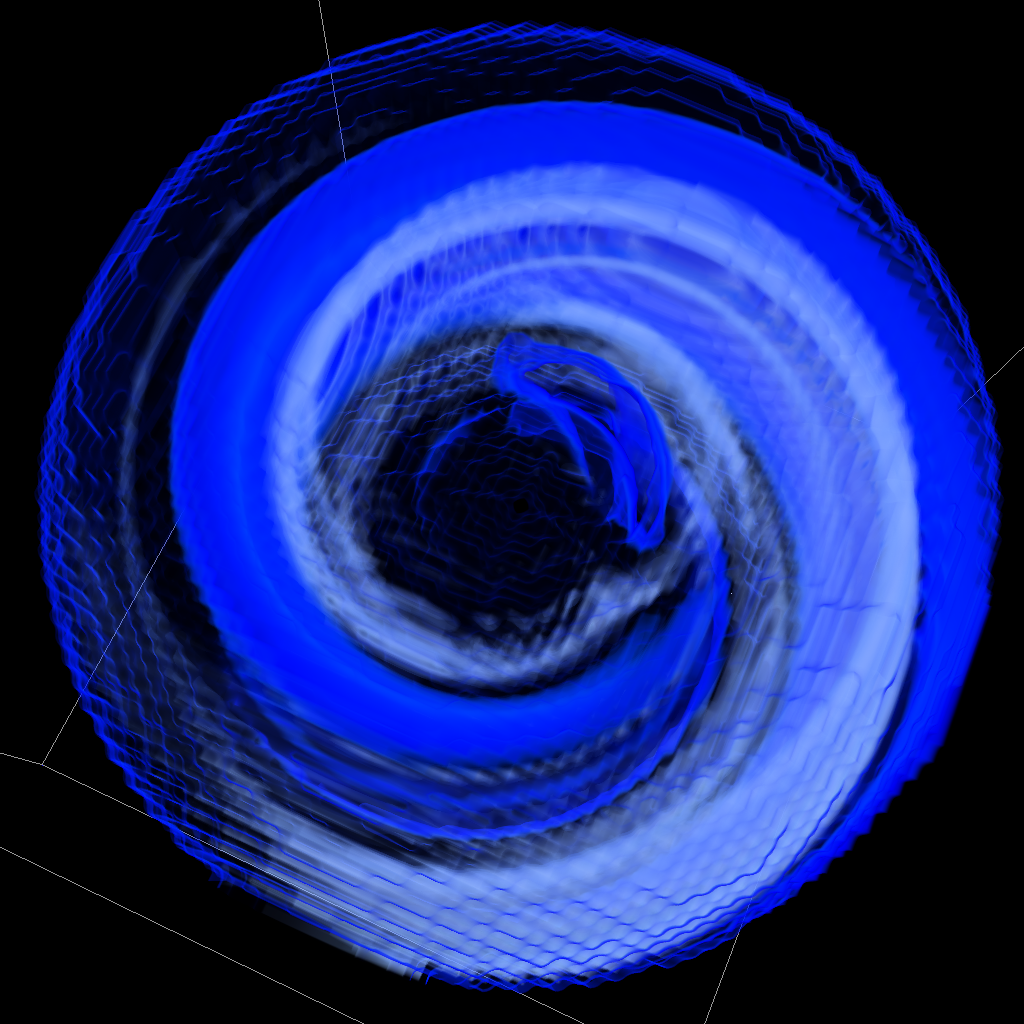
\includegraphics[width=0.32\linewidth]{figures/cube_64.png}}
	\subfigure[Resampled (double resolution)]{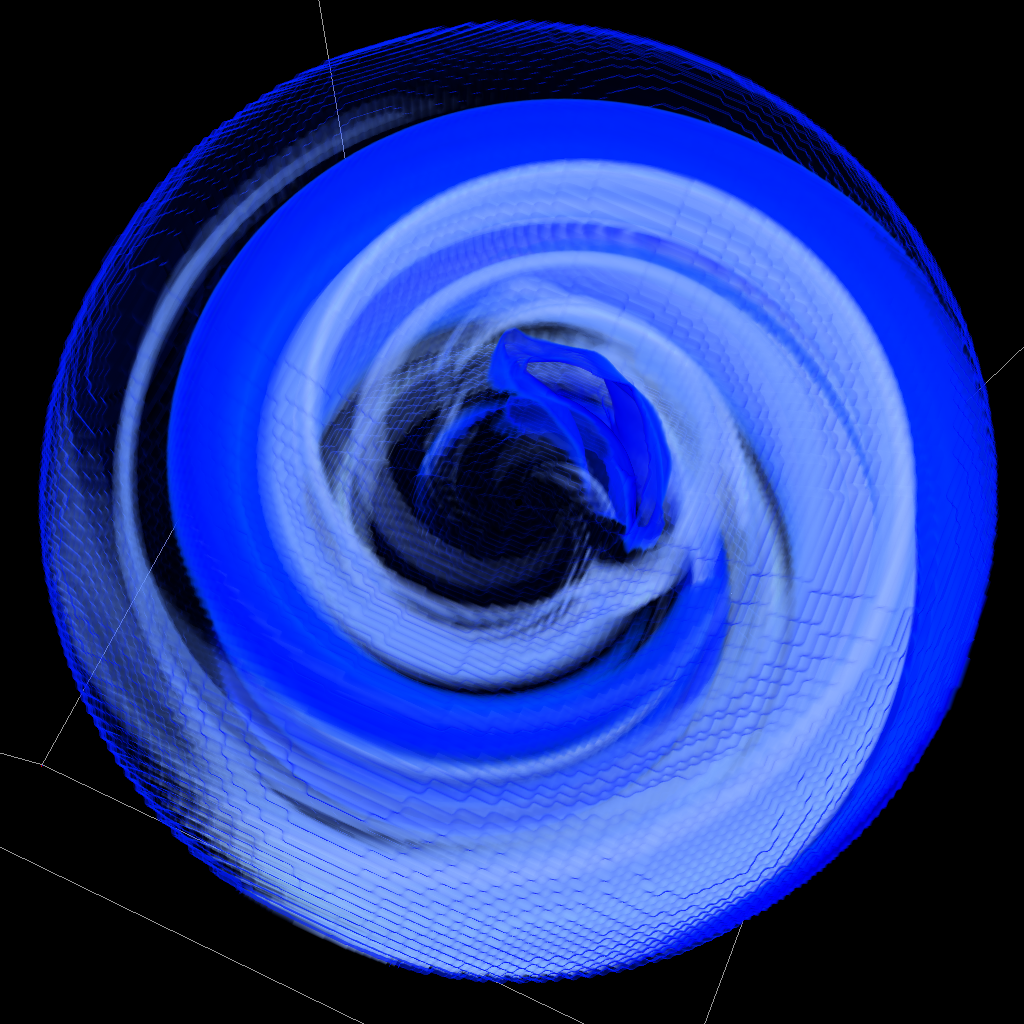
\includegraphics[width=0.32\linewidth]{figures/cube_128}}
	\caption{Using the native spherical coordinates (a) to perform the raycasting enables resolving structures in the outer regions of the volume with much greater detail compared to the resampled volume with the same data size (64 $\times$ 64 $\times$ 64) (b). Even if the size of the resampled volume is increased 8-fold (c) the effect still persists.}
	\label{fig:teaser}
}

\maketitle

\begin{abstract}
We are investigating the effects of performing tradition volumetric raycasting on datasets that have an innate spherical symmetry. These datasets are frequently created by using simulations that operate by solving a model with a spherical symmetry. Usually, these models are resampled to a regular Cartesian grid prior to isosurface or raycasting-based rendering. This operation does not only leave a great part of the volume unused, it is also oblivious to difference in resolution between the inner core and the outer regions of the model. Both drawbacks can be resolved by storing the results of the simulation in the native spherical coordinates and performing the volume lookup in the same coordinate system. Furthermore, we will present our findings of using a radius-dependent integration step length in the rendering pipeline to account for denser data values close to the origin, thus, allowing data-aware importance sampling.

%\begin{classification} % according to http://www.acm.org/class/1998/
%\CCScat{Computer Graphics}{I.3.3}{Picture/Image Generation}{Line and curve generation}
%\end{classification}

\end{abstract}

\section{Introduction}
\label{sec:introduction}
Simulations are a necessary and important tool that have found widespread use in the computational subfields of many different domains. Among these domains are computational fluid dynamics, hydrodynamics, simulations in the material sciences, and many more and the results of these simulations allow scientists to gain invaluable insight into their respective object of interest. Visualizing and understanding fine structures in this kind of data is of primary interest to the domain specialists.

In the process of designing the simulation, the expert can consider, among others, the utilized coordinate systems. Normally, this choice reflects some innate symmetry own to the specific problem at hand. These various symmetries are exploited by the simulation designer to speed up the calculation. Using the spherical coordinate system is one of the possible symmetries that can be employed in the solution whenever the underlying problem shows a behavior that is of spherical symmetry. The details will be explained in Section~\ref{sec:background}, but within such a coordinate system, each point is identified not by the Cartesian coordinates $(x,y,z)$, but by the radius, longitude, and latitude $r,\, \phi,\, \theta$. Please note that there exist different notations about spherical coordinates and that we stick to the convention used in physics, i.\,e., $\phi$ is the azimuthal angle and $\theta$ is the polar angle, in the remainder of the paper. One integral attribute of this coordinate system is that there is an unequal spatial distribution of computed points; Figure~\ref{fig:resamplingerror} shows this effect using the 2-dimensional equivalent, the polar coordinates.

In this work, we will refer to a \emph{Cartesian volume} whenever the three axes of a rectangular volume denote Cartesian $(x,y,z)$ coordinates, and \emph{spherical volume} if $(r,\, \theta,\, \phi)$ is used as principal axes. Please note that the stored volume is of rectangular shape in both cases.

\begin{figure}
	\centering
	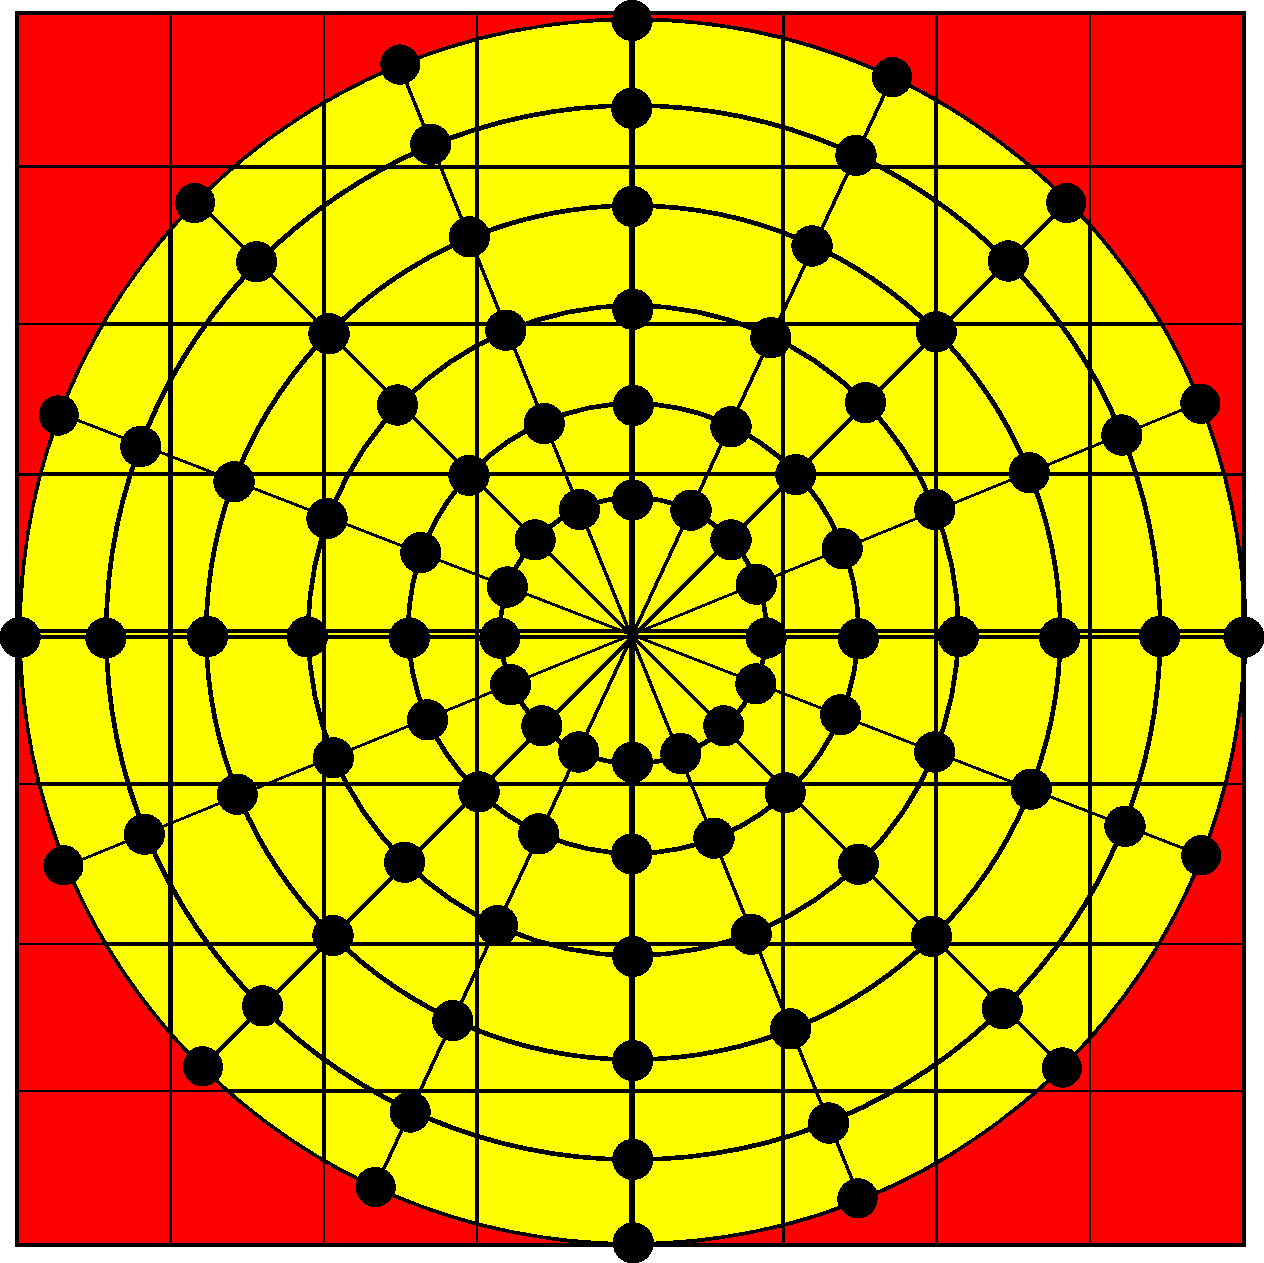
\includegraphics[width=0.75\columnwidth]{figures/spherical_resampling.pdf}
	\caption{Using a non-Cartesian coordinate system can lead to a non-uniform spatial distribution of computed points. If points are distributed with an equidistant $\phi$ value, the euclidean area of a shell close to the center is much smaller than in the outer areas. Resampling the coordinate system does not take the uneven distribution into account and leads to undersampling in the outer regions and/or oversampling close to the center. The image shows this as the density of values in the resampled, rectilinear volume is not constant. Furthermore, approximating a sphere by a rectangular bounding box wastes storage space in the outer regions as depicted by the red colored area.}
	\label{fig:resamplingerror}
\end{figure}

To visualize the results of simulation runs, one common approach is to resample the data, given in spherical coordinates, to a Cartesian grid. This allows an easier processing by the state-of-the-art rendering techniques and enables efficient rendering, but has the major drawback of not taking the $r$-dependent point distribution into account (see Figure~\ref{fig:resamplingerror}). This leads to either of two problems; if the resampling rate chosen such that the resulting volume will be comparable in size to the spherical volume, areas close to the center will be undersampled whereas areas in the outer shells will be oversampled, thus creating an overall bad resolution. If the resampling rate is chosen high enough to resolve important details in the center, much space will be wasted in the outer shells because those points will be oversampled even further. In addition to that, representing a sphere using a rectangular bounding box leaves much of the space unused and wastes storage space even further (see Figure~\ref{fig:resamplingerror} and Section~\ref{sec:memory}).

In this work we propose a method that, while perfoming the raymarching in Cartesian coordinates, transforms each sampling point into spherical coordinates to fetch the correct data value. Interpolating the data in the spherical coordinate system  allows the interpolated values to stay true to the spherical symmetry the data was originally computed in. Using this approach, we can achieve a rendering at the full resolution without increasing or wasting memory. Furthermore, since we have access to the radial component during the raymarching and the data density is dependent on the radius, we can achieve an importance-based sampling rate that will take smaller steps in areas with more available data.

\section{Related Work}
\label{sec:relatedwork}
To the authors' knowledge, there is no article in the literature employing fundamental spherical symmetry in datasets and evaluating the impact on rendering time and quality due to this coordinate transform. The closest work that has been published deals with 4D ultra-sound visualization, in which the data is stored as a time-varying 3-dimensional polar coordinates format~\cite{bruder11}.

Alternative ways to render these datasets have been proposed. If the underlying simulation is performed on a finite element grid, it is intuitive to render the elements directly and many techniques have been presented to achieve this, c.f.~\cite{ueff10,bock12} among others.

Furthermore, multiresolution schemes, which are usually applied to enable rendering of big datasets, can be easily adjusted to allow for efficient storage of these datasets. This technique would mitigate the problems that arise from radius-dependent voxel densities. A number of techniques have been proposed on this topic, e.g.~\cite{lamar99,weiler00,ljung06}.

\section{Background}
\label{sec:background}
The data that we use throughout the paper have been created by the Community Coordinated Modeling Center at Goddard Space Flight Center at NASA. It is the result of a time-dependent, 3D magnetohydrodynamic model of the heliosphere, called ENLIL. In this simulation a recorded coronal mass ejection (CME), see Figure~\ref{fig:cme}, is used as the initial condition for a fluid dynamics solver that takes the plasma mass, momentum, energy density, and the magnetic fields into account to solve for the movement of high energy partices. CMEs often occur due to reconnection of magnetic field lines that transform the Sun's magnetic potential energy into kinetic energy that accelerates charged particles into interplanetary space. The study of CMEs is a highly important part in the context of Space Weather; "[Space weather] refers to conditions on the Sun and in the solar wind, magnetosphere, ionosphere, and thermosphere that can influence [...] technological systems and endanger human life or health." \cite{SpaceWeather95}. Concrete knowledge of the CMEs and solar wind has direct impact on the safety of space missions, satellites, power grids, and others.

\begin{figure}
	\centering
	\subfigure[Coronal Mass Ejection] {
		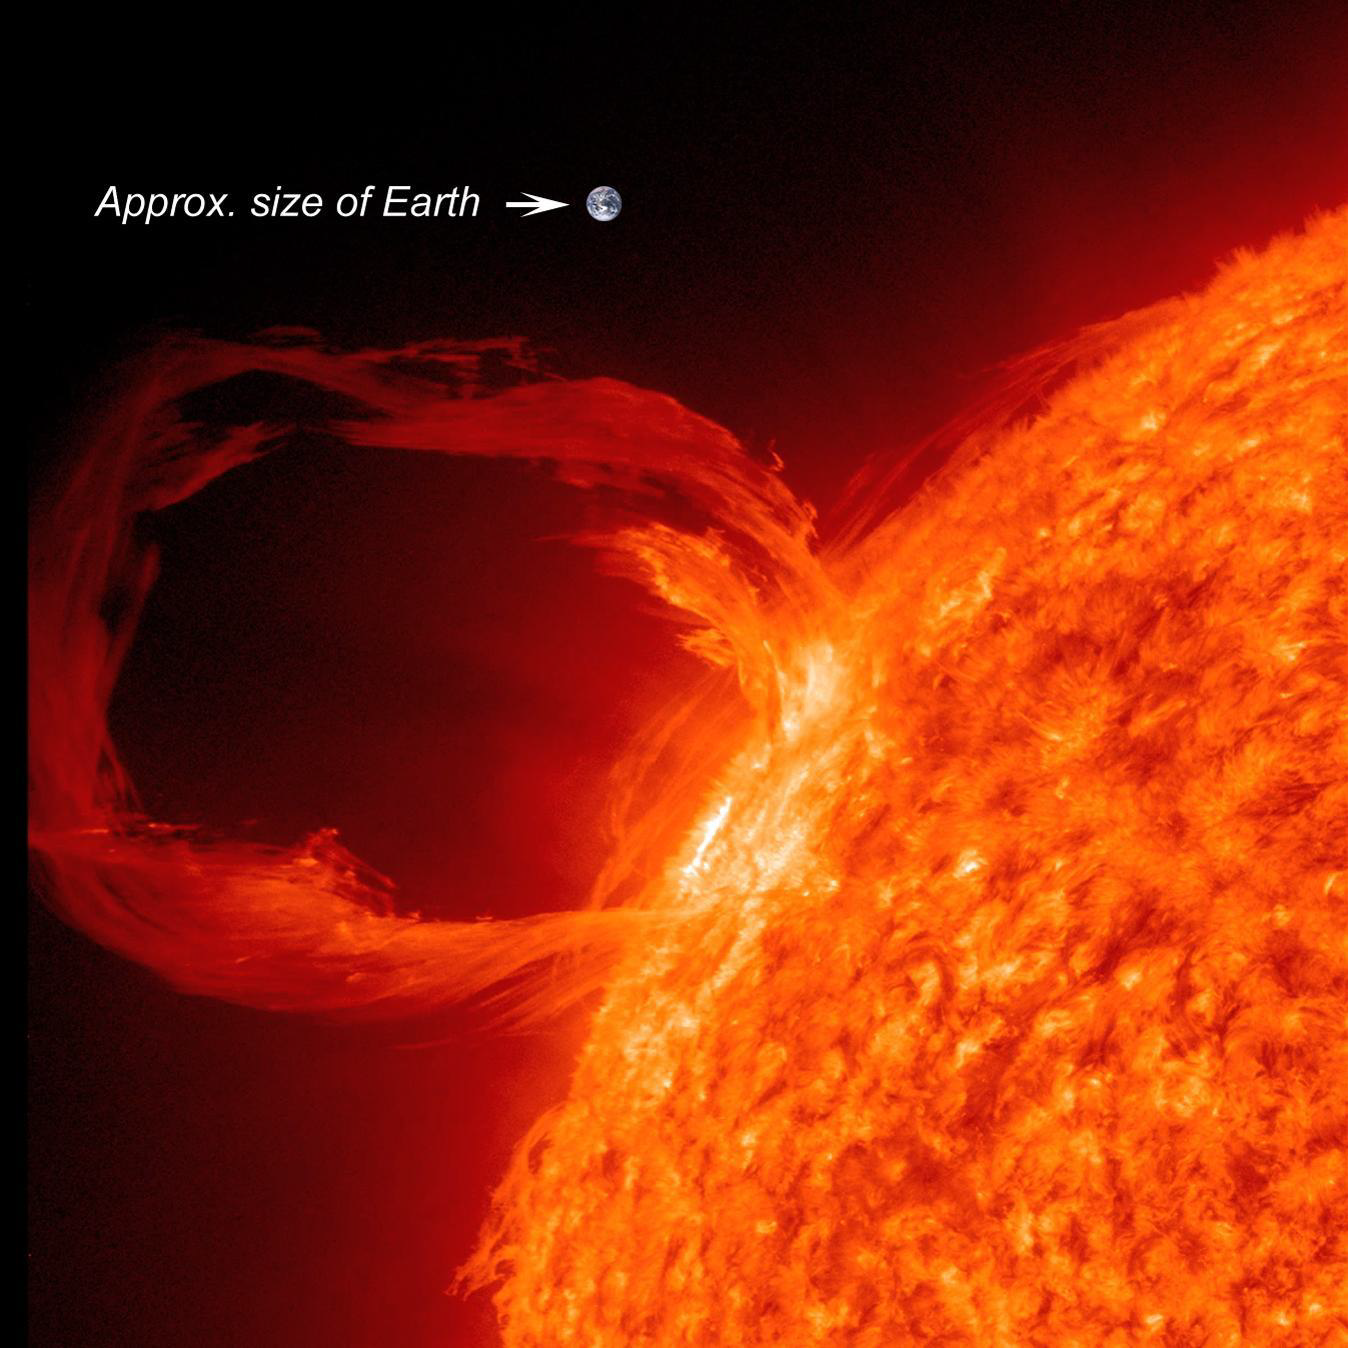
\includegraphics[width=0.47\columnwidth]{figures/soho.png}
		\label{fig:cme}
	}
	\subfigure[CCMC Runs on Request] {
		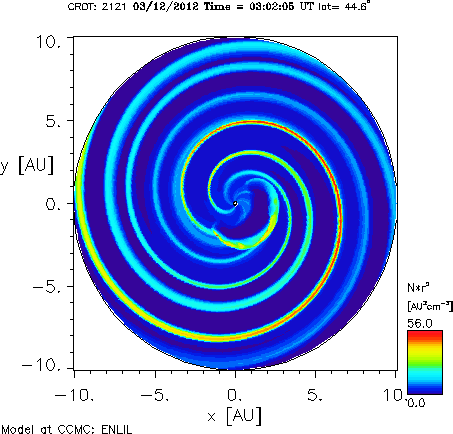
\includegraphics[width=0.47\columnwidth]{figures/ccmc_ror.png}
		\label{fig:ror}
	}
	\caption{(a) A Coronal Mass Ejection event as seen from the Solar and Heliospheric Observatory. In the image, the Earth is shown as a reference for the size of the CME event. (b) An output from the CCMC's Run on Request feature as it is in use by the scientist at the moment.}
\end{figure}

The ENLIL simulation is performed natively on a spherical grid with the Sun in the origin and the model reaching up to about 10 AU, which is about the orbit of Jupiter. Figure~\ref{fig:ror} shows an output of one of the visualization tools that are currently used by the domain experts.

\section{Spherical Raycasting}
\label{sec:spherical}
\begin{algorithm}
\begin{algorithmic}[1]
\REQUIRE Entry point $e_0$ and exit point $e_1$ in world coordinates
\REQUIRE Sampling step size $t_{incr}$
\STATE $t_{length} \gets \| e_1 - e_0 \|$
\STATE $e_{dir} \gets \left( e_1 - e_0 \right) / t_{length}$
\STATE $t \gets 0$
\WHILE {$t \leq t_{length}$}
	\STATE $pos \gets e_0 + t \cdot e_{dir}$
	\STATE $r \gets \| pos \|$
	\STATE $\theta \gets \cos^{-1}(pos.z / r)$
	\STATE $\phi \gets \tan^{-1}(pos.y, pos.x)$
	\STATE $value \gets sampleVolume(r, \theta , \phi)$
	\STATE Classification and front-to-back blending
	\STATE $t \gets t + t_{incr}$
\ENDWHILE
\ENSURE Composited color value

\end{algorithmic}
\caption{Our modified ray casting algorithm}
\label{alg:raycasting}
%\SetAlgoLined
%\KwData{Entry point $e_0$ and exit point $e_1$ of the ray}
\end{algorithm}

Given a spherical volume, i.\,e., a rectangular volume where the principal axes are the radius $r$, longitude $\phi$, and latitude $\theta$, we perform a modified version of the raycasting scheme introduced by \cite{Kr}. An overview of the algorithm is presented in Algorithm~\ref{alg:raycasting}. The Entry-Exit points can be set up using two different methods; based on the radial extent of the volume and a known voxel spacing, we can construct a cuboidal bounding box with texture coordinates mapped to the range $[0,1]$ for each dimension. The alternative is to generate a spherical bounding box with the same texture coordinate mapping. As this choice is not important to the rest of the pipeline, we defer the discussion of these two methods to their respective section~\ref{sec:entryexit}.

Using the entry-exit points, a straight ray in world space is constructed, just as in regular volume raycasting. During the raymarching, each Cartesian sampling point on the view ray is transformed into the spherical coordinate system using the equations
$$r = \sqrt{x^2 + y^2 + z^2} \; \; \; \; \; \; \; \phi = atan\left(\frac{y}{x}\right) \; \; \; \; \; \; \; \theta = acos\left(\frac{z}{r}\right)$$
and the resulting tuple $(r, \phi, \theta)$ is used to look up the value in the spherical volume. Hence, we will refer to this tuple as look-up values.

\subsection{Interpolation}
\label{sec:interpolation}
\begin{figure}
	\centering
	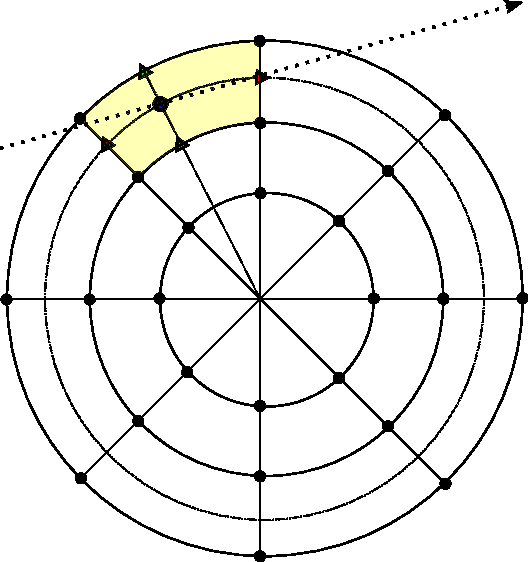
\includegraphics[width=0.75\columnwidth]{figures/spherical_interpolation.pdf}
	\caption{This figure shows a 2-dimensional representation of the interpolation scheme that we employ on the spherical data. By using hardware-supported trilinear interpolation on the spherical volume, we achieve an interpolation behavior that is identical with a spherical linear interpolation (SLERP). By linearly interpolating the angle $\phi$, the interpolated values are located on a concentric circle, thereby staying true to the underlying spherical structure of the data. In the example we want to retrieve the value at the blue sampling location. While the (linear) radial interpolation provides the green values, the interpolation in $\phi$ produces the red values. In this case it is important to note that the weighting factor is not based on the euclidean distance between the red values and the blue sample point, but the weighting factor is regard along the concentric arc connecting the two points. The same holds true for the second angle in the 3-dimensional case.}
	\label{fig:interpolation}
\end{figure}

As the transformed sampling point will not be exactly at one voxel position, interpolation of the surrounding values has to be performed to get a correct value. In the case of a regular Cartesian volume, trilinear interpolation (or any other interpolation scheme) would be used to achieve this. However, as the underlying data is of spherical nature, linear interpolation along Cartesian axes would lead to interpolation artefacts as exact sample positions are lost during the resampling. In the case of a spherical volume, there exist two native ways of interpolating; positional interpolation or value interpolation.

In \emph{positional interpolation}, the visual appearance of trilinear interpolation in a  Cartesian volume is duplicated. The algorithm is as follows: the sampling point's neighbors in the Cartesian coordinate system are generated and each of the neighbors is transformed into the spherical coordinates. These transformed values are used to look up the data values in the spherical volume and regular interpolation of these values is performed. This interpolation scheme results in the same result as trilinear interpolation performed directly on the Cartesian volume.

In \emph{value interpolation}, the neighbor generation is performed in the spherical volume instead of the Cartesian world coordinate system. After transforming the single sample position into spherical coordinates, the direct neighbors in the spherical volume are computed and a regular trilinear interpolation is performed on these values. The result of this interpolation scheme is similar to using a Spherical Linear Interpolation (SLERP). A schematical overview of method is shown in Figure~\ref{fig:interpolation}.

As the value interpolation stays truer to the underlying data, we use this method of interpolation for the rest of this paper.

\subsection{Memory Footprint}
\label{sec:memory}
To transform the native model calculation from spherical to Cartesian coordinates, it has to be surrounded by a cuboid bounding box and resampled to a regular grid. As the data is of spherical nature, it will only occupy a sphere in the center of this volume whereas no data values exist for the rest and can therefore be considered wasted memory.

Given a radius $r$, the volume of a sphere is given as: $V_s = \frac{4}{3}\pi r^3$, whereas the volume of a cube surrounding a sphere is $V_c = (2r)^3 = 8r^3$. The amount of useful memory in the cuboid volume is therefore given by: $V_s /V_c = \frac{\pi}{6} \approx 0.52$. This means that for a spherical volume, about 48\% of the stored memory does not contain any data and is therefore wasted.

\subsection{Precision}
\label{sec:precision}
Apart from the obvious waste of memory, the more severe drawback of resampling the spherical data to a regular grid is the loss in precision. For the resampling the user has to choose a constant step size that is used for each part of the bounding box. As shown in Figure~\ref{fig:resamplingerror}, the data value density for spherical models is higher close to the center of the sphere and it decreases towards the outer layers.

As the distribution of data values in the spherical volume is independent of $r$ and the volume of a spherical sector is proportional to $1/r^3$, the data value density exerts a $1/r^3$ proportionality as well.

\subsection{Entry-Exit Points}
\label{sec:entryexit}
As described earlier about 48\% of the rectangular bounding box is empty of data values and can therefore be ignored in the ray casting process. We implemented a two specialized empty-space skipping algorithms suited for the spherical data distribution.

The first algorithm uses a spherical rendering primitive instead of a rectangular cube. The world coordinates are mapped to the texture coordinates for each of the vertices that constitute the sphere. The drawback of this method, however, is that the sphere can only be approximated by piece-wise continuous surfaces and traditional methods create approximations that are smaller than the sphere would have been. We, therefore, did not pursue this method further.

The second algorithm uses a common ray-sphere intersection calculation to refine the entry point $e_0$ and exit point $e_1$ before applying the raycasting. The impact on performance by this method is investigated in Section~\ref{sec:performance}.

\subsection{Dynamic Step Length}
\label{sec:dynamicstep}
It is possible to exploit the $1/r^3$ dependency in data density in the rendering step to perform data-aware importance sampling along the view ray. As the data density decreases in the outer areas of the sphere, it is sufficient to sample the view ray less dense. Vice versa, it is beneficial to increase the sampling step size closer to the origin. This technique is not limited to the case of a spherical volume, but it can be trivially integrated as the radial distance to the center is already available.

We implemented the dynamic step length by replacing line 11 of Algorithm~\ref{alg:raycasting} with:
$$ t \gets t_{incr} \cdot \left( s \cdot r + 1 - m \right)^3 $$
where $s$ and $m$ are parameters to control the behavior of the adaptive sampling, which can be modified by the user to balance the trade-off between performance and rendering accuracy by flattening or increasing the $1/r^3$ dependency.

\section{Performance}
\label{sec:performance}
\begin{figure}
	\centering
	\subfigure[Spherical Raycasting] {
		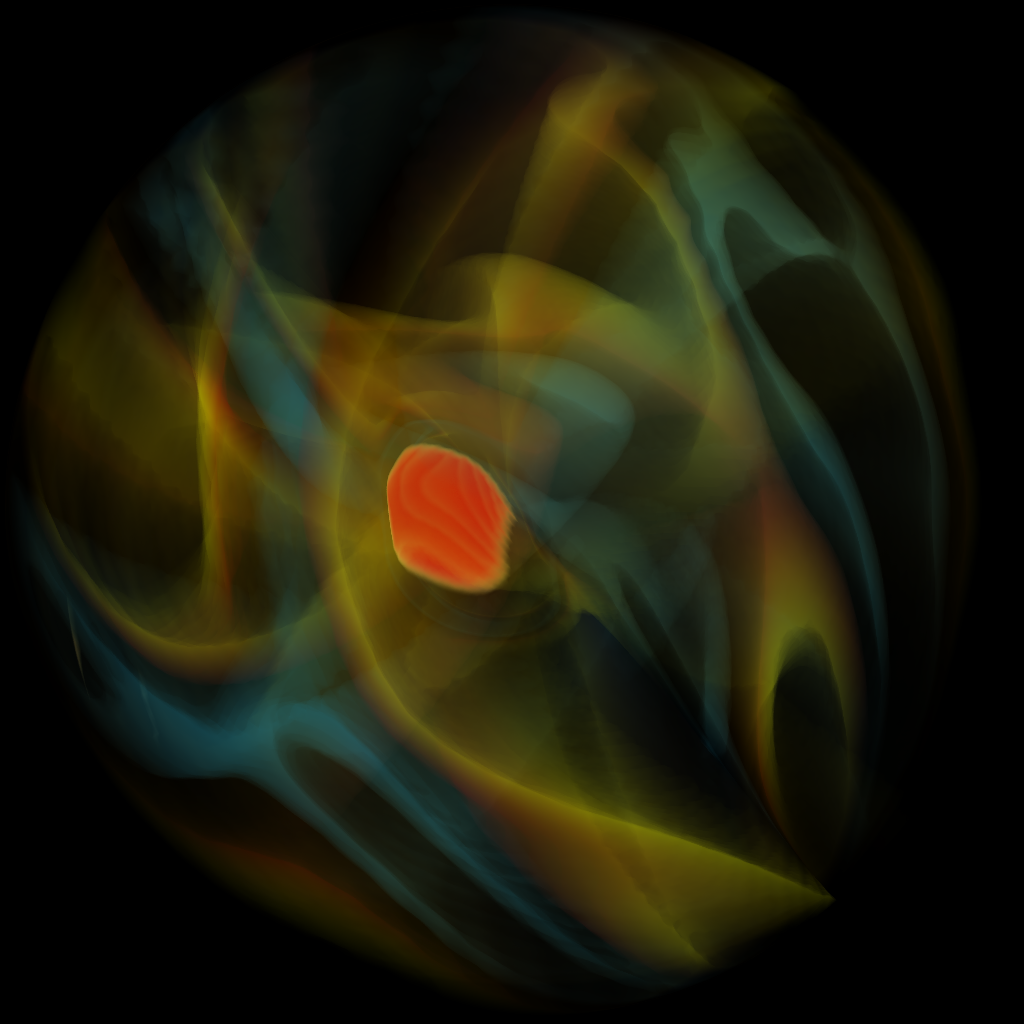
\includegraphics[width=0.45\columnwidth]{figures/performance-spherical.png}
		\label{fig:performnce:spherical}
	}
	\subfigure[Cartesian Raycasting] {
		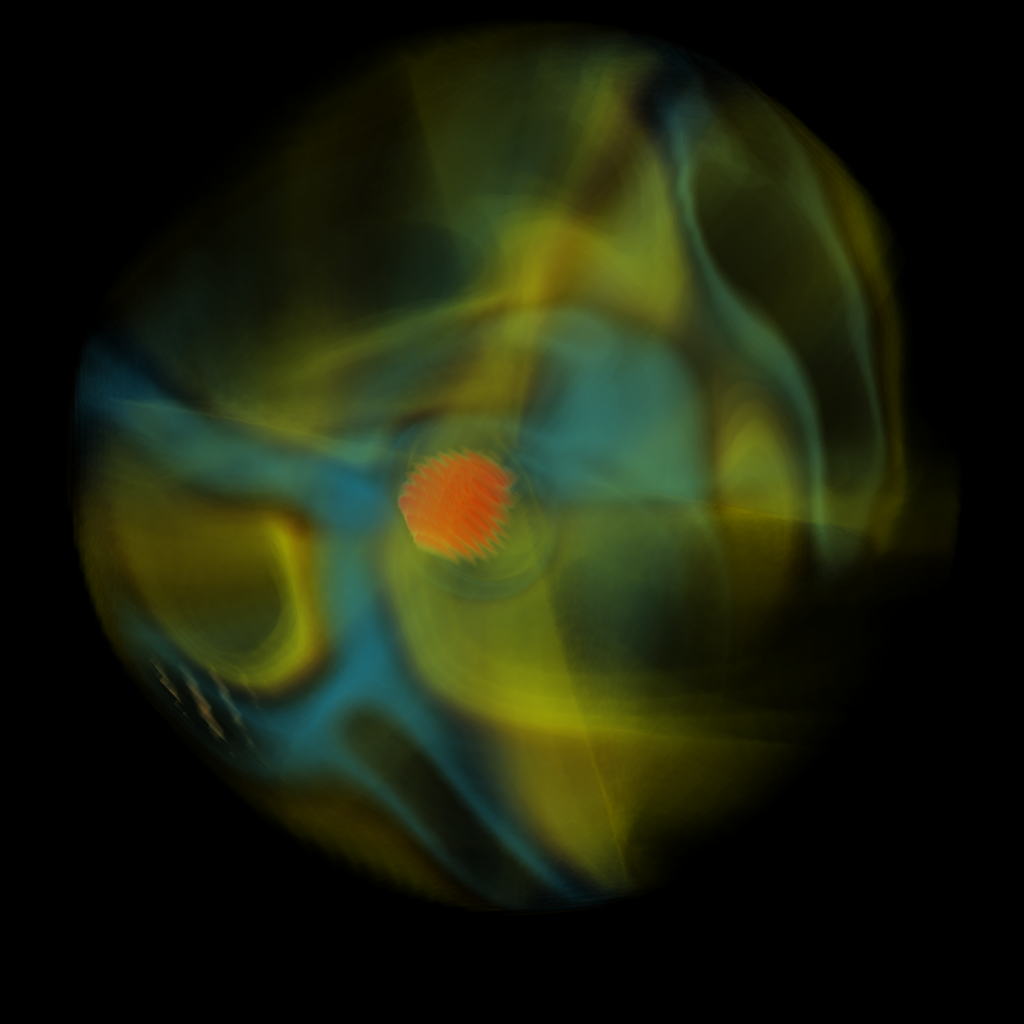
\includegraphics[width=0.45\columnwidth]{figures/performance-cartesian.png}
		\label{fig:performance:cartesian}
	}
	\caption{One of the volumes and transfer functions that were used in the performance measurements. In this case, the spherical rendering (a) achieved 19 \emph{fps}, while the Cartesian rendering (b) achieved 24 \emph{fps}.}
	\label{fig:performance}
\end{figure}

\begin{figure}
	\centering
	\subfigure[No Adaptive Raycasting] {
		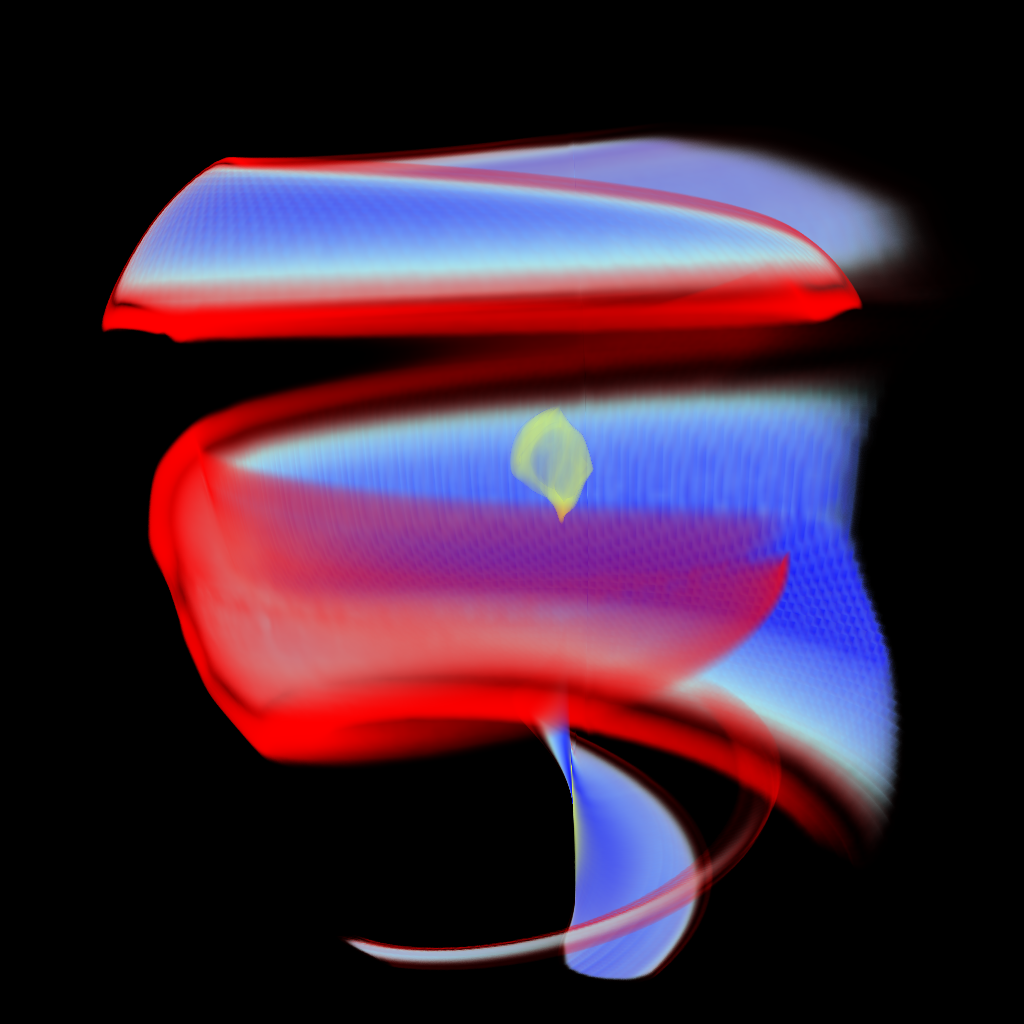
\includegraphics[width=0.45\columnwidth]{figures/performance-adaptive-no.png}
	}
	\subfigure[$s = 0.15$ and $m = 0.1$] {
		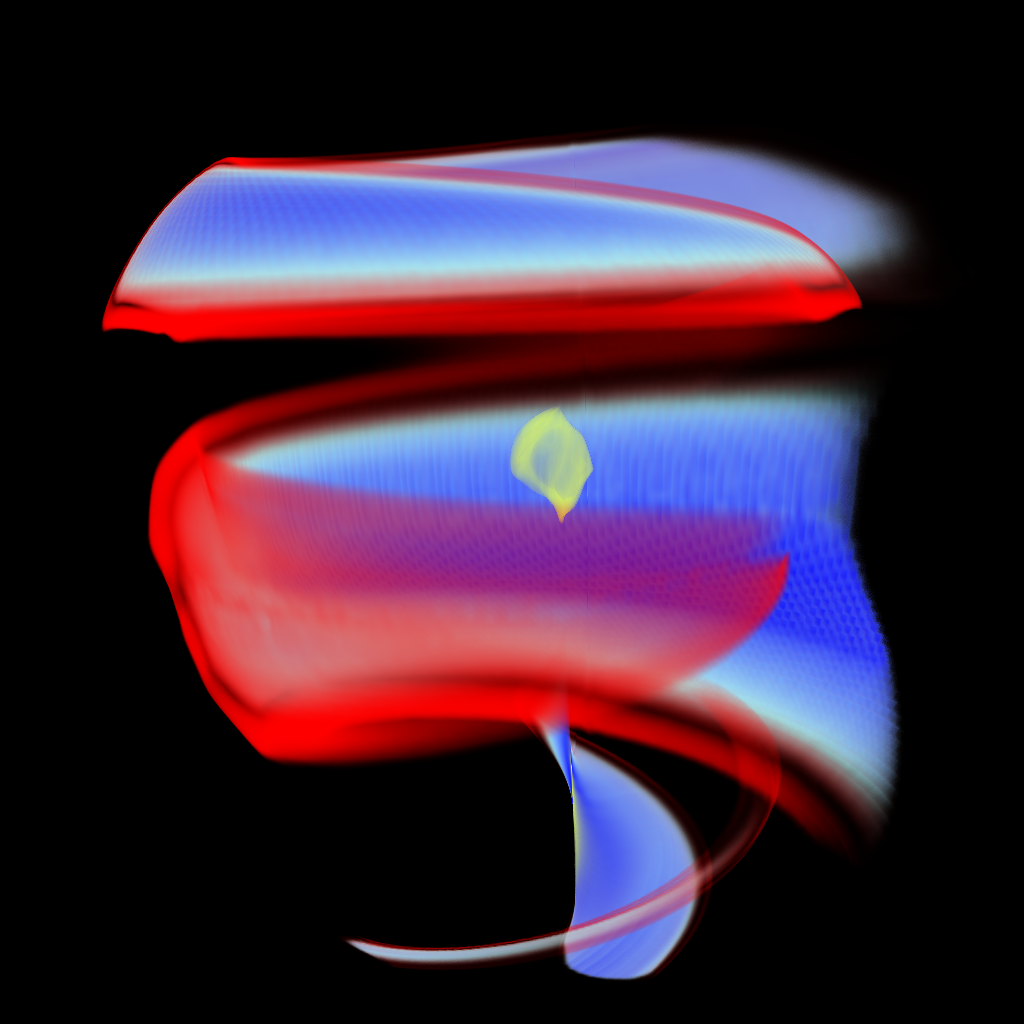
\includegraphics[width=0.45\columnwidth]{figures/performance-adaptive-015-01.png}
	}
	\subfigure[$s = 0.5$ and $m = 0.1$] {
		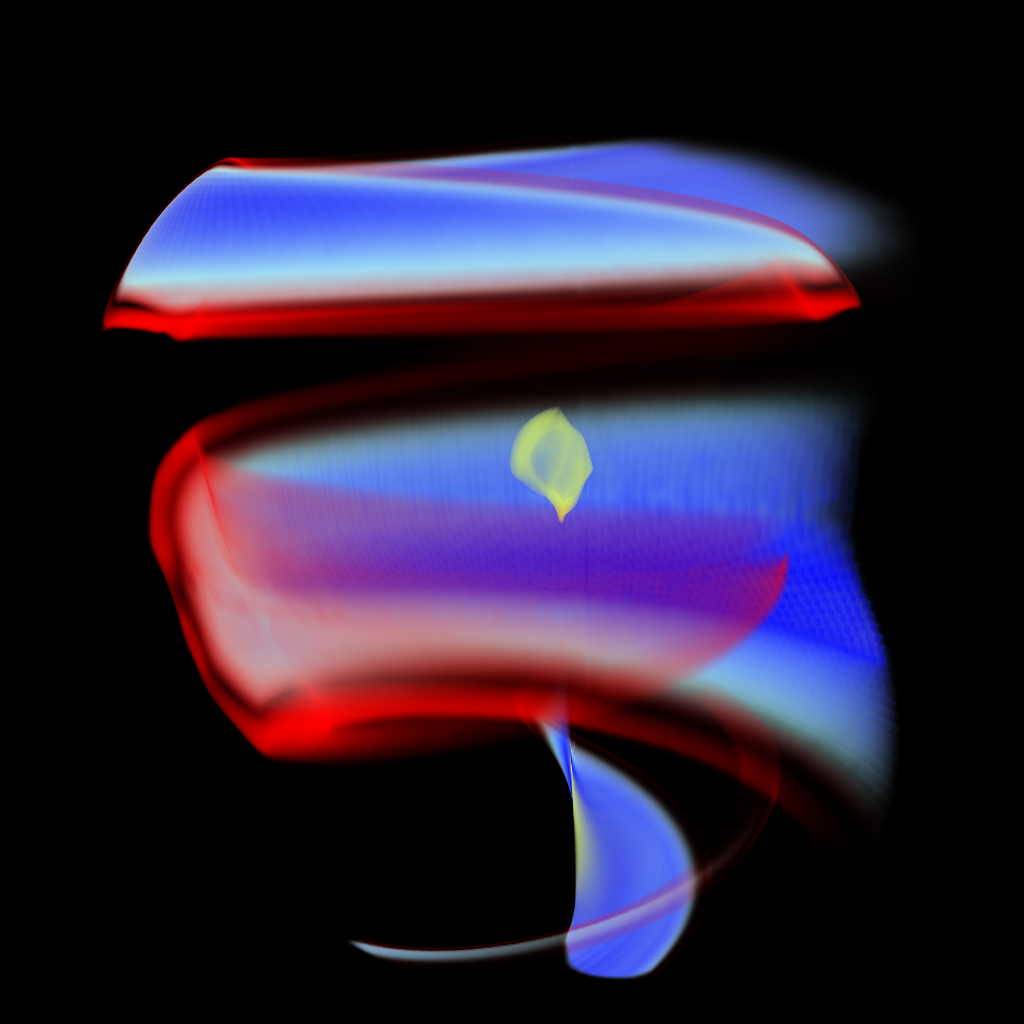
\includegraphics[width=0.45\columnwidth]{figures/performance-adaptive-05-01.png}
	}
	\subfigure[$s = 0.5$ and $m = 0.5$] {
		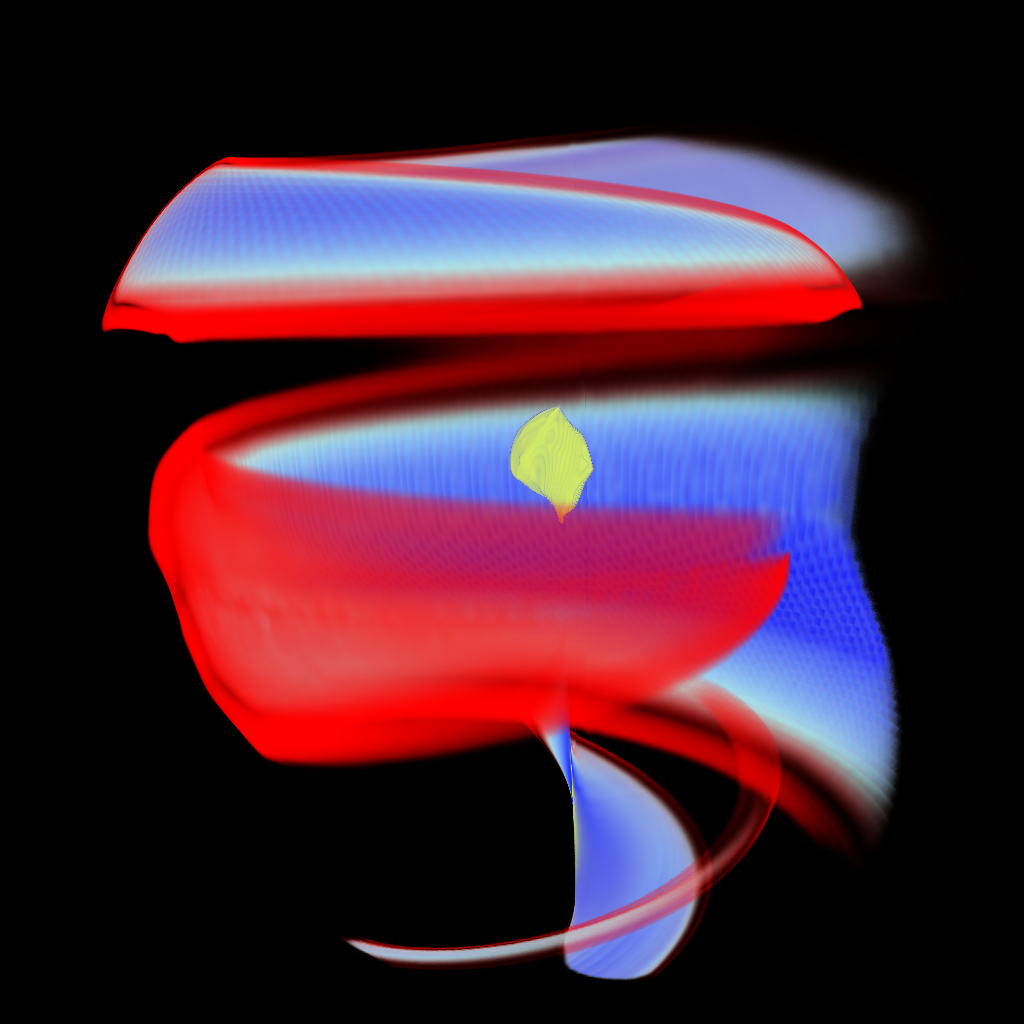
\includegraphics[width=0.45\columnwidth]{figures/performance-adaptive-05-05.png}
	}
	\subfigure[$s = 0.85$ and $m = 0.1$] {
		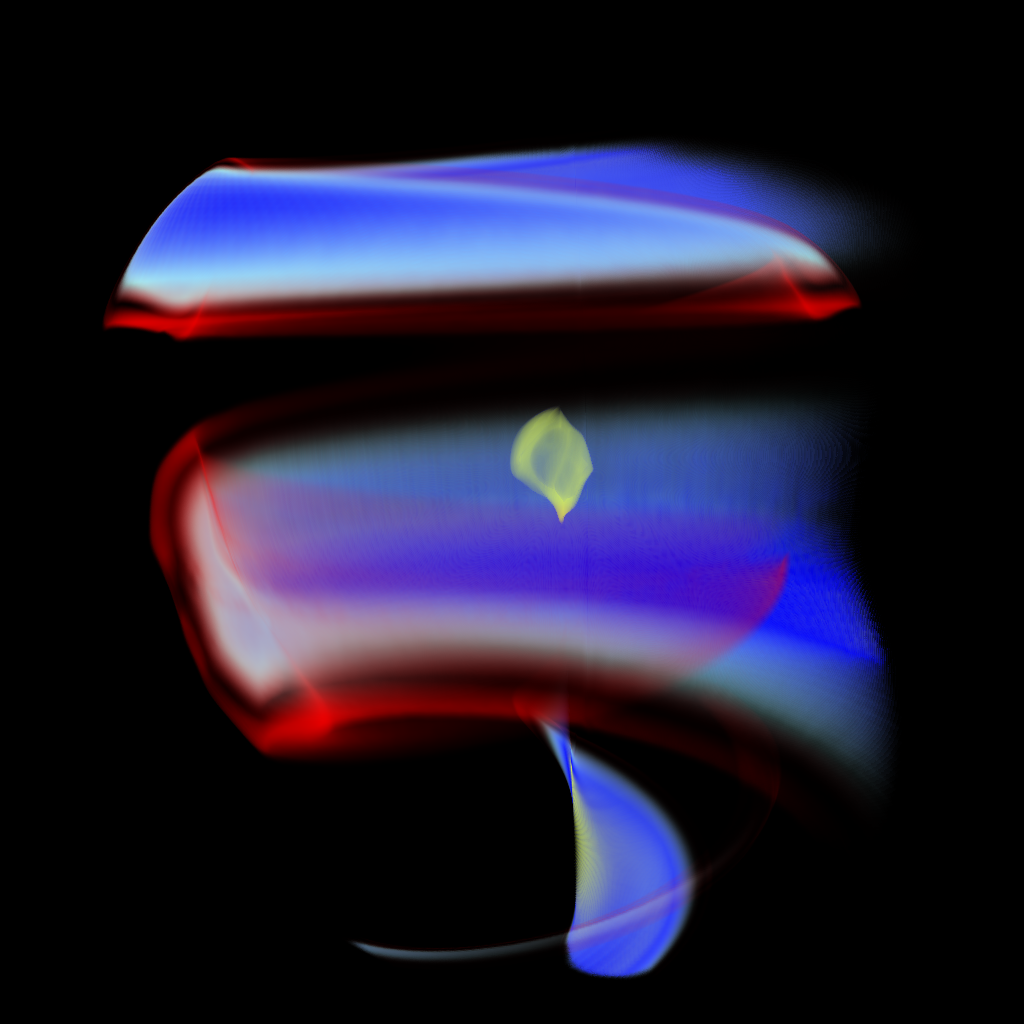
\includegraphics[width=0.45\columnwidth]{figures/performance-adaptive-085-01.png}
	}
	\subfigure[$s = 0.85$ and $m = 0.5$] {
		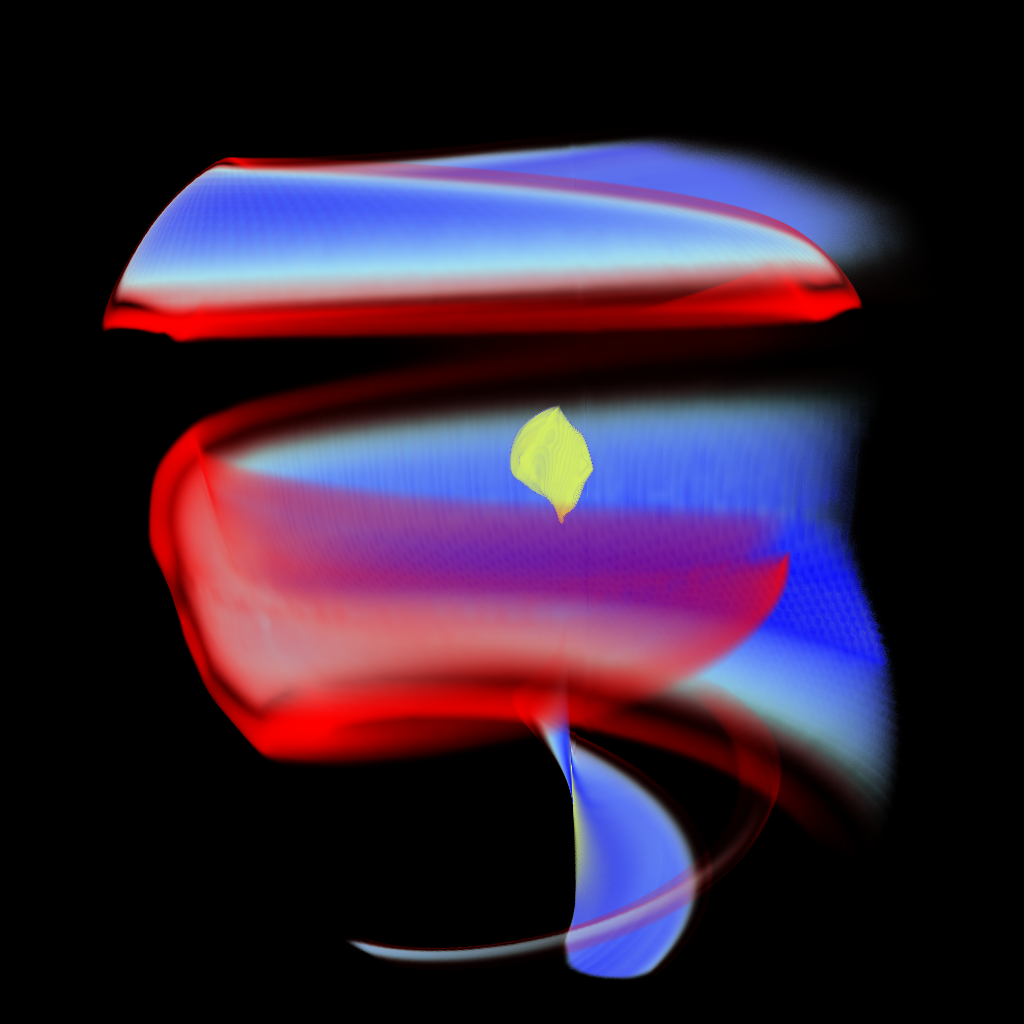
\includegraphics[width=0.45\columnwidth]{figures/performance-adaptive-085-05.png}
	}
	\caption{Comparing the various user-defined parameters controlling the slope and minimum values of the $1/r^3$ adaptive sampling.}
	\label{fig:performance:adaptive}
\end{figure}

We carried out performance tests on an nVidia Geforce GTX 580 graphics card to investigate the impact of our method. We compared our method to the straight forward Cartesian raycasting to investigate the impact of the additional coordinate transformation. Furthermore, we examined the performance impact of a some parameter setups for the adaptive sampling.

It is expected that, compared to Cartesian raycasting, there is reduced performance due to the coordinate transformation prior to the volume lookup. We created a Cartesian volume and a spherical volume of sizes $128 \times 128 \times 128$ and performed the respective ray casting method on these volumes. During these tests with various transfer functions (see Figure~\ref{fig:performance}), we found an average of about 20\% performance decrease, when performing spherical ray casting.

Because of the subjective nature of the result of the adaptive sampling, it is difficult to perform conclusive performance tests on this method. We chose some representative parameter values that are explained in Figure~\ref{fig:performance:adaptive} and Table~\ref{tab:performance}. The tests show that it is possible to vary the framerate and visual appearance on both ends of the quality/speed spectrum to suit the user's rendering needs.

\begin{table}[b]
  \caption{Performance measurements of user-defined parameters for $1/r^3$ adaptive sampling. All performance measurements were done with the same transfer function on the same $256 \times 256 \times 256$ volume.}
  \label{tab:performance}
  \begin{center}
    \begin{tabular}{|c|c|r|}
      \hline
      $s$ parameter & $m$ parameter & fps \\
      \hline
      \multicolumn{2}{|c|}{no adaptive} & 11.85 \\
      0.15 & 0.1 & 12.15 \\
      0.5  & 0.1 & 22.83 \\
      0.5  & 0.5 & 7.00 \\
      0.85 & 0.1 & 36.88 \\
      0.85 & 0.5 & 12.97 \\
      \hline
    \end{tabular}
  \end{center}
\end{table}

\section{Conclusion}
\label{sec:conclusion}
In this paper we presented and elaborated on our method to render spherical volumes. Instead of resampling a computational model, given with spherical symmetry, to a Cartesian grid and using state-of-the-art rendering techniques, we allow for rendering that operates directly on the data addressed by using the spherical coordinate system. This technique avoids the problem of having a mismatch between the constant sampling rate for the resampling and the $1/r^3$ proportionality in the data value density. This avoids visual artifacts that would be very prominent in small volumes otherwise. It, furthermore, enables more efficient memory usage as the resampling results in about 50\% unused memory.

We carried out performance tests to investigate the impact of the additional coordinate system change on the rendering speed. In our test cases we found that the coordinate change inflicts a performance hit of about 20\% on the total rendering time. To accommodate for this performance hit, we employed an adaptive sampling scheme that makes use of the varying voxel densities to achieve a importance-based sampling of the volume data.

\section*{Acknowledgments}
The presented concepts have been realized using the Voreen framework (www.voreen.org). Simulation results have been provided by the Community Coordinated Modeling Center at Goddard Space Flight Center through their public Runs on Request system (http://ccmc.gsfc.nasa.gov). The CCMC is a multi-agency partnership between NASA, AFMC, AFOSR, AFRL, AFWA, NOAA, NSF and ONR.

\bibliographystyle{eg-alpha}

\bibliography{literature}

%-------------------------------------------------------------------------
\newpage


%\begin{figure*}[tcb]
%  \centering
%  \mbox{} \hfill
  % the following command controls the width of the embedded PS file
  % (relative to the width of the current column)
%  \includegraphics[width=.3\linewidth]{sampleFig}
  % replacing the above command with the one below will explicitly set
  % the bounding box of the PS figure to the rectangle (xl,yl),(xh,yh).
  % It will also prevent LaTeX from reading the PS file to determine
  % the bounding box (i.e., it will speed up the compilation process)
  % \includegraphics[width=.3\linewidth, bb=39 696 126 756]{sampleFig}
%  \hfill
%  \includegraphics[width=.3\linewidth]{sampleFig}
%  \hfill \mbox{}
%  \caption{\label{fig:ex3}%
   %        For publications with color tables (i.e., publications not offering
      %     color throughout the paper) please \textbf{observe}: 
         %  for the printed version -- and ONLY for the printed
           %version -- color figures have to be placed in the last page.
%           \newline
   %        For the electronic version, which will be converted to PDF before
      %     making it available electronically, the color images should be
         %  embedded within the document. Optionally, other multimedia
%           material may be attached to the electronic version. }
%\end{figure*}

\end{document}

